\chapter{Security Analysis}
\label{sec:security_analyse}

% Ist das zentrale Kapitel der Arbeit. Hier werden das Ziel sowie die
% eigenen Ideen, Wertungen, Entwurfsentscheidungen vorgebracht. Es kann
% sich lohnen, verschiedene Möglichkeiten durchzuspielen und dann
% explizit zu begründen, warum man sich für eine bestimmte entschieden
% hat. Dieses Kapitel sollte - zumindest in Stichworten - schon bei den
% ersten Festlegungen eines Entwurfs skizziert werden.
% Es wird sich aber in einer normal verlaufenden
% Arbeit dauernd etwas daran ändern. Das Kapitel darf nicht zu
% detailliert werden, sonst langweilt sich der Leser. Es ist sehr
% wichtig, das richtige Abstraktionsniveau zu finden. Beim Verfassen
% sollte man auf die Wiederverwendbarkeit des Textes achten.

% Plant man eine Veröffentlichung aus der Arbeit zu machen, können von
% diesem Kapitel Teile genommen werden. Das Kapitel wird in der Regel
% wohl mindestens 8 Seiten haben, mehr als 20 können ein Hinweis darauf
% sein, daß das Abstraktionsniveau verfehlt wurde.

%\ldots design \ldots

%\todo{write design}

This chapter aims to analyze the potential vulnerabilities in Vanilla Quark, through which an adversary can obtain access to confidential information of an application. The first section defines the threat model(Section~\ref{sec:Threat_model}). 
Subsequently, this chapter scrutinizes the Vanilla Quark's security from the perspective of the Open Container Initiative (OCI) interface (Section~\ref{sec:security_analysis}).
This chapter aims to analyze the potential vulnerabilities in Vanilla Quark, through which an adversary can obtain access to confidential information of an application. The first section defines the threat model (Section~\ref{sec:Threat_model}). 
Subsequently, this chapter scrutinizes Vanilla Quark's security from the perspective of the Open Container Initiative (OCI) interface~\cite*{oci-runtime-spec} (Section~\ref{sec:security_analysis}).

\section{Threat model}
\label{sec:Threat_model}
We employ the OWASP application threat modeling methodology\cite*{OWASP_Threat_Modeling} to create a threat model comprising four aspects: actors, assets, external dependencies, and attack surface. 

\textbf{Actors.} Our model involves the cloud provider and the tenant. While the cloud provider is accountable for providing the hardware and software necessary for running and orchestrating applications, the tenant distrusts the cloud provider 
in a confidential computing environment. Therefore, any software components within the cloud infrastructure - Kubernetes control plane\cite*{k8s}, containerd\cite*{containerd}, and hypervisor are untrusted.

\textbf{Assets.} Our objective is to secure the Kubernetes workload (application) itself, i.e., preserving the integrity of the application binary and its dependencies, maintaining the confidentiality and integrity of the application's data during runtime, and protecting the secrets provided to the application by its owner.

\textbf{External Dependencies.} We assume that the Guests, including Qkernel and Kubernetes workloads, operate within an encrypted virtual machine. This prevents malicious hypervisor(Qvisor) or powerful cloud operators from accessing the workload's sensitive 
data through guest memory and registers. Furthermore, we exclude attacks related to denial of service~\cite*{DOS_ATTACK}, side channels~\cite*{217454}, networks, or file systems.


\textbf{Attack Surface.} We focus on attacks occurring on the OCI interface~\cite*{oci-runtime-spec}. As the management of workloads is the cloud provider's responsibility, it must have a means of accessing workloads for orchestration, even if the 
workloads are running within a TEE. Although the OCI runtime specification offers this possibility, it exposes a new attack surface for an adversary to probe workloads' secrets. Additionally, since the OCI  implementation in the guest interacts with 
the host through the Hypercall, Qcall, or Ucall interface, we also considered attacks from this interface.


\section{Security Analysis}
\label{sec:security_analysis}

This section provides an in-depth security analysis of the implementation of the OCI runtime interface within Quark.  Notably, Qlib serves solely as a development concept since Qlib code is incorporated into the Qkernel and Qvisor binaries during 
the compilation. Therefore, the following sections use Qkernel and Qvisor to refer to the respective binaries containing the qlib code.

The subsequent subsections thoroughly examine the potential pitfalls of the OCI implementation in Quark in the context of confidential computing from seven perspectives. These include application secrets deployment, handling  STDIO of guest user 
space process, command execution and terminal allocation, paravirtualized file system sharing, guest system call,  guest kernel arguments, and guest logging system. The Design chapter further proposes mechanisms to mitigate these vulnerabilities.


This section provides a security analysis of the OCI runtime interfaces~\cite*{oci-runtime-spec} implemented within Quark. Notably, Qlib serves solely as a development concept since its code is incorporated into the Qkernel and Qvisor binaries 
during the compilation. Therefore, the following sections use Qkernel and Qvisor to refer to the respective binaries containing the Qlib code.

The subsequent sections examine the potential pitfalls of the OCI implementation in Quark in the context of confidential computing from seven perspectives:

\begin{itemize}
  \item Application secrets deployment.
  \item Handling STDIO of guest user space process.
  \item Command execution and terminal allocation.
  \item Para-virtualized file system sharing.
  \item Guest system call.
  \item Guest kernel arguments.
  \item Guest logging system. 
\end{itemize}

The Chapter~\cite*{sec:design} further proposes mechanisms to mitigate the vulnerabilities we found in this chapter.


\subsection{Application Secrets Deployment}
\begin{figure}[H]
    \centering
    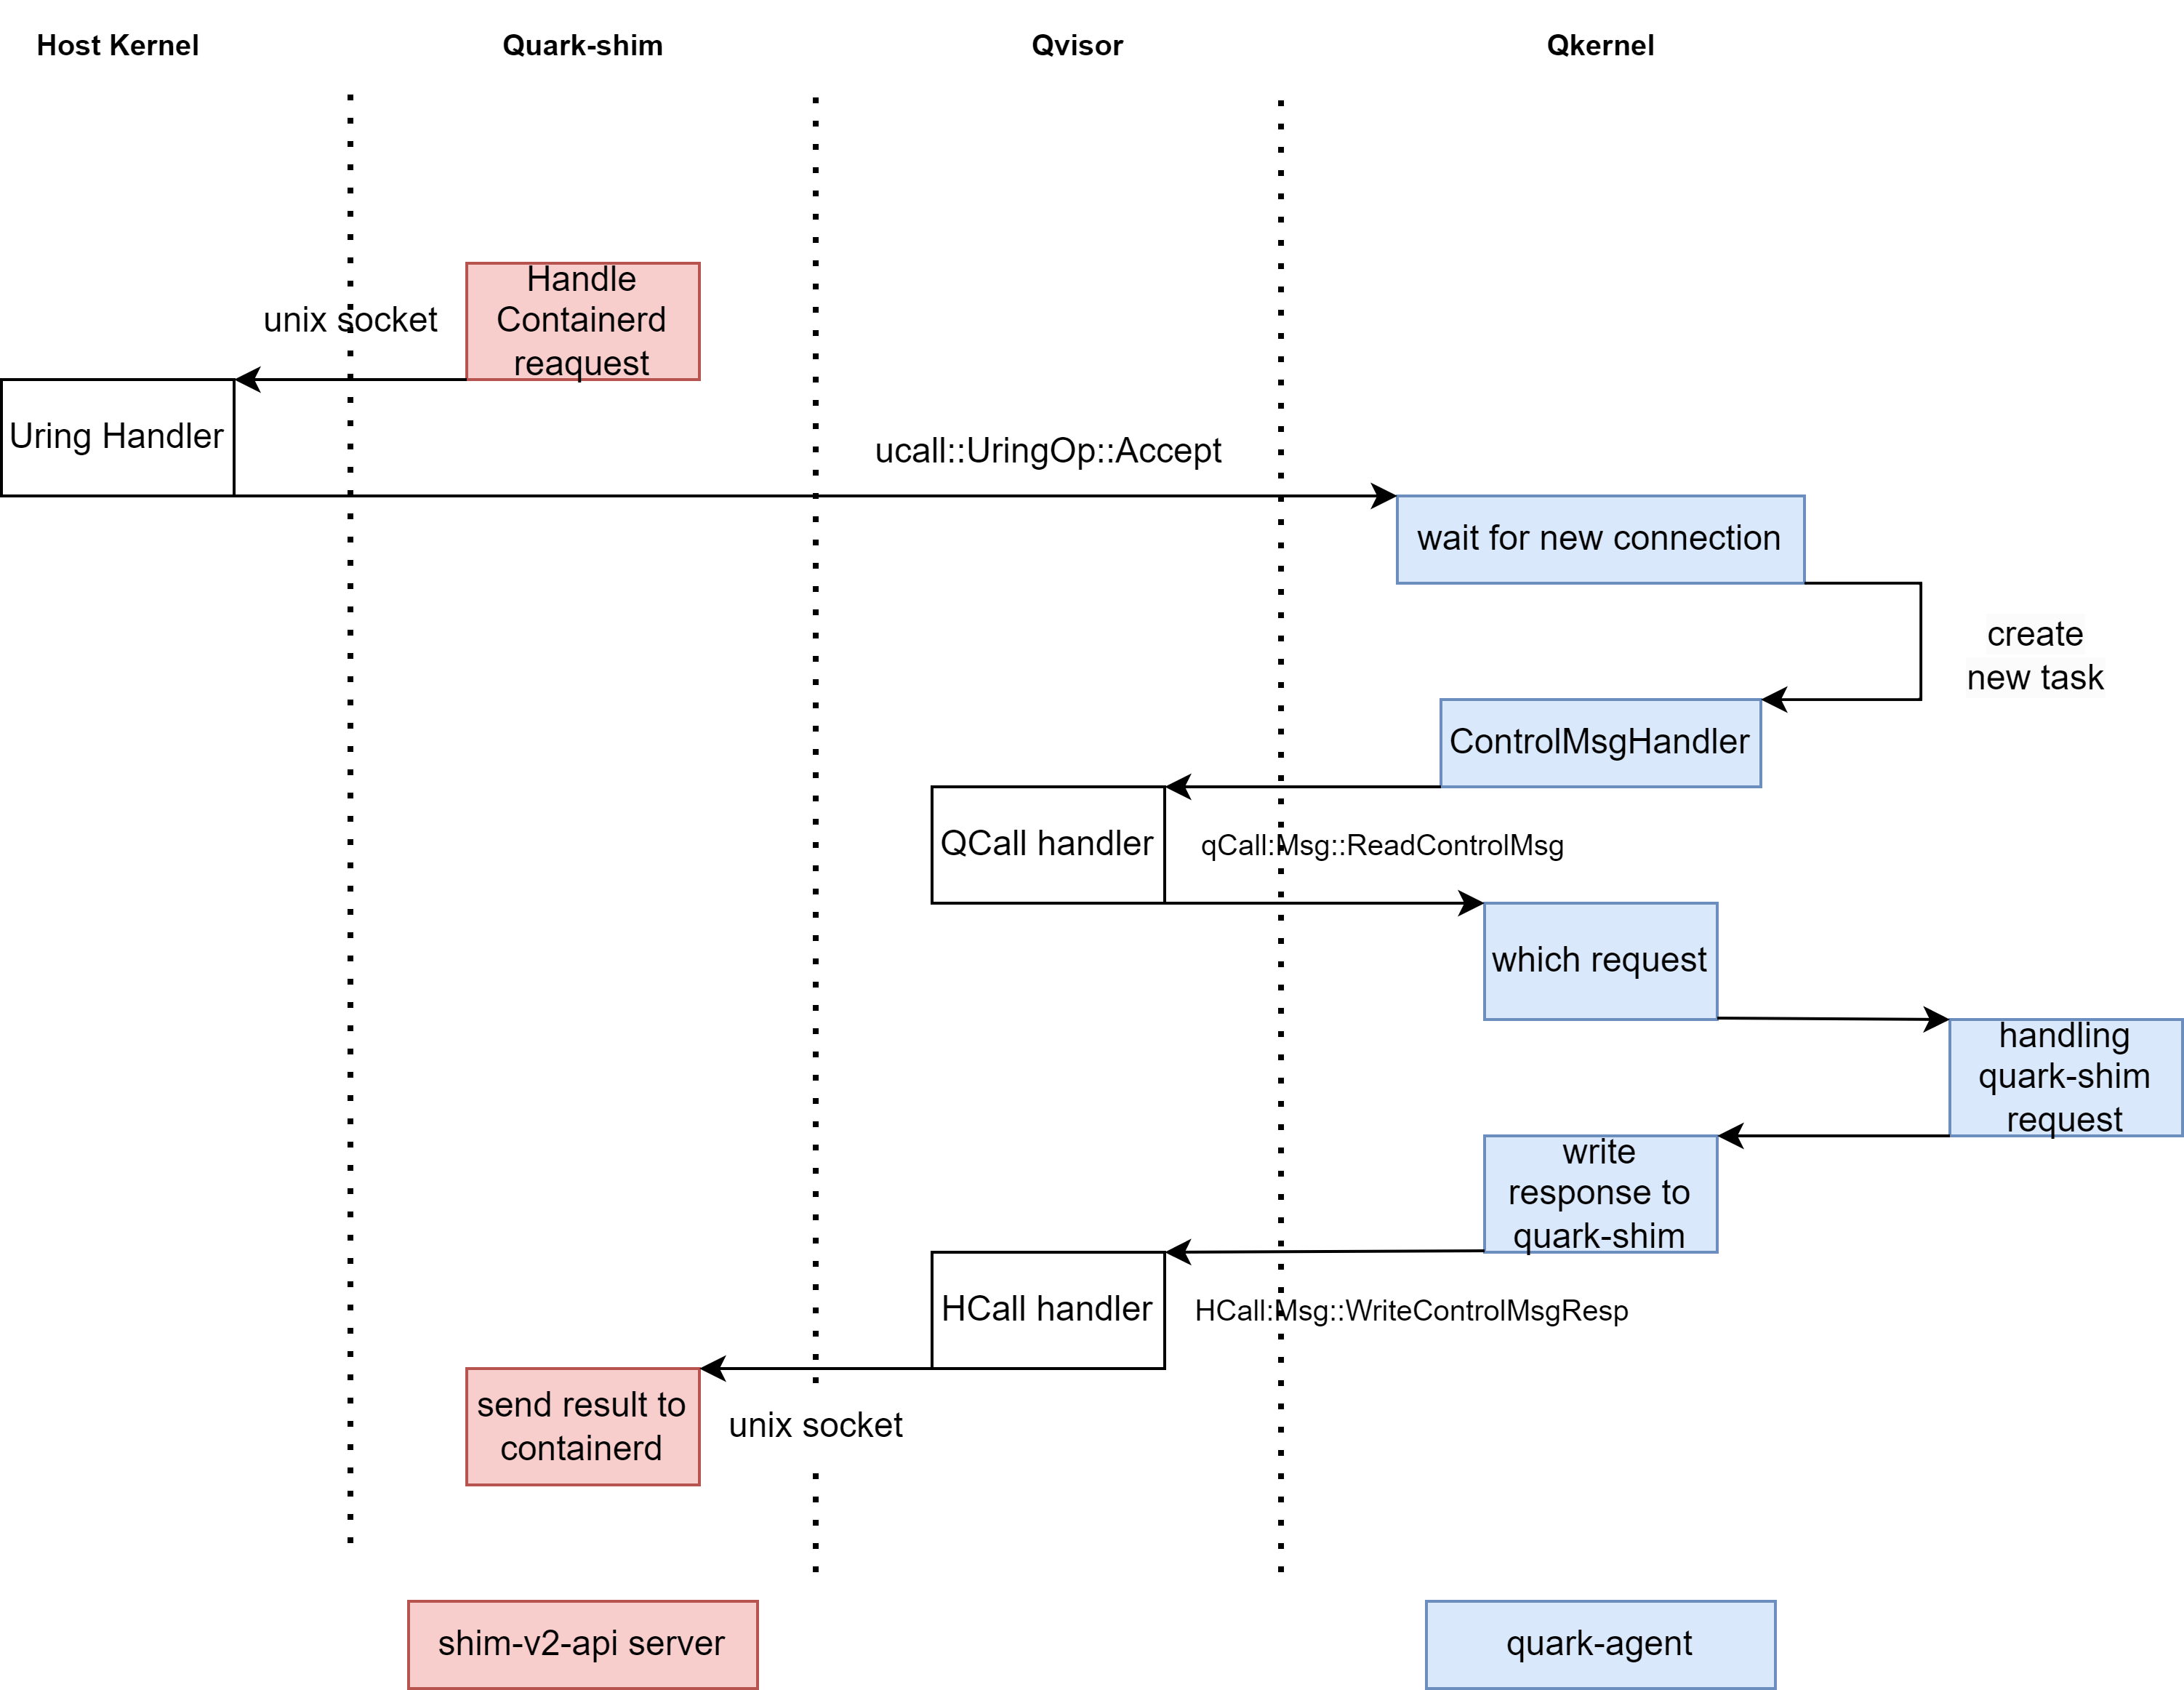
\includegraphics[width=0.8\textwidth]{images/quark-agent-work-flow.png}
    \caption[Quark Agent Workflow]{Quark agent Workflow. The Quark agent is located in the qkernel. It is responsible for receiving requests from Quark-shim, like creating application processes, creating exec processes, deleting application processes, etc.}
    \label{fig:quark_agent_work_flow}
\end{figure}


\textbf{Untrusted Kubernetes and the Quark shim process manage and deploy application secrets}. 
These secrets may be injected into the application through command line arguments, mounted files, or environment variables. When deploying the application, Containerd~\cite*{containerd} generates an Application Bundle and transmits it via the 
shim v2 API~\cite*{shim_v2} to the shim-v2-API server in the Quark-shim process. This bundle contains the rootfs of the application along with an OCI-compatible config.json file~\cite*{oci-runtime-spec}. Quark-shim creates the root filesystem for 
the container on the host side, mounts the file type secret, and establishes the process specification. This specification contains the command line type and the environment variable type secrets.  The Quark-shim then uses the Unix socket to 
request the Quark agent in the Qkernel to create an application process based on this process specification. The workflow is shown in Figure~\ref*{fig:quark_agent_work_flow}.


 Quark-agent operates as a socket server accepting connection requests from the Quark shim through Ucall::Uringop::accept(). These requests include creating and deleting application processes, creating an exec process, etc. Upon receiving a request 
 from the Quark-shim to create an application (exec) process, the Uringop::accept returns a host file descriptor that contains the process specification. As the Quark agent in the Qkernel cannot read its contents directly, it 
 employs Qcall: Msg::ReadControlMsg to request the Qvivor to read the file descriptor and return the specification. The specification provides metadata for creating a process, including command line arguments, environment variables, the type of 
 STDIO (terminal or normal IO), and the host file descriptor for transmitting data from/to the process STDIO. Based on the specification, Quark-agent creates a guest user process. Specifically, the command line arguments and the environment 
 variables are pushed to the process stack, and the STDIO of the process is set accordingly to the type of STDIO specified in the specification. Further details about the process’s STDIO can be found in section~\ref*{sec:security_analyse_STDIO}.


 It is imprudent to Kubernetes to manage application secrets (file type, command line type, environment variable type secrets) and deploy them through Containerd and Quark shim, since they are untrusted. In particular, individuals with access to 
 the cluster can use the kubectl to view or modify the Kubernetes-managed secrets. Additionally, an adversary can manipulate Containerd and Quark shim during application deployment to tamper with the application secrets by modifying the application 
 bundle. Besides, when Quark-agent uses the Qcall interface to request Qvisor to read the process specification containing secrets, Qvisor could potentially steal or modify these secrets. To this end, we suggest offloading secret deployment and 
 management from Kubernetes, Quark-shim, and Qvisor. For a detailed explanation of the mitigation, please refer to section~\ref*{sec:design_Secret_Uploading}.

\subsection{Guest User Space Process STDIO}
\label{sec:security_analyse_STDIO}

The Quark agent loads the corresponding binary and initiates a guest user-space process for handling the request of either creating an application or executing a command (kubectl exec)~\cite*{k8s}. Thus, Quark handles the application process STDIO 
in the same way as it handles the exec process STDIO. For instance, when Containerd~\cite*{containerd} wishes to create an exec process in Qkernel, three named pipes are created for the process's standard input, output, and error. These are then 
passed to Quark-shim via the quark-shim-v2 API~\cite*{shim_v2} along with other metadata. Quark-shim then employs these data to create the exec request's process specification. 


\begin{figure}[ht] 
    \begin{subfigure}[b]{0.5\linewidth}
      \centering
      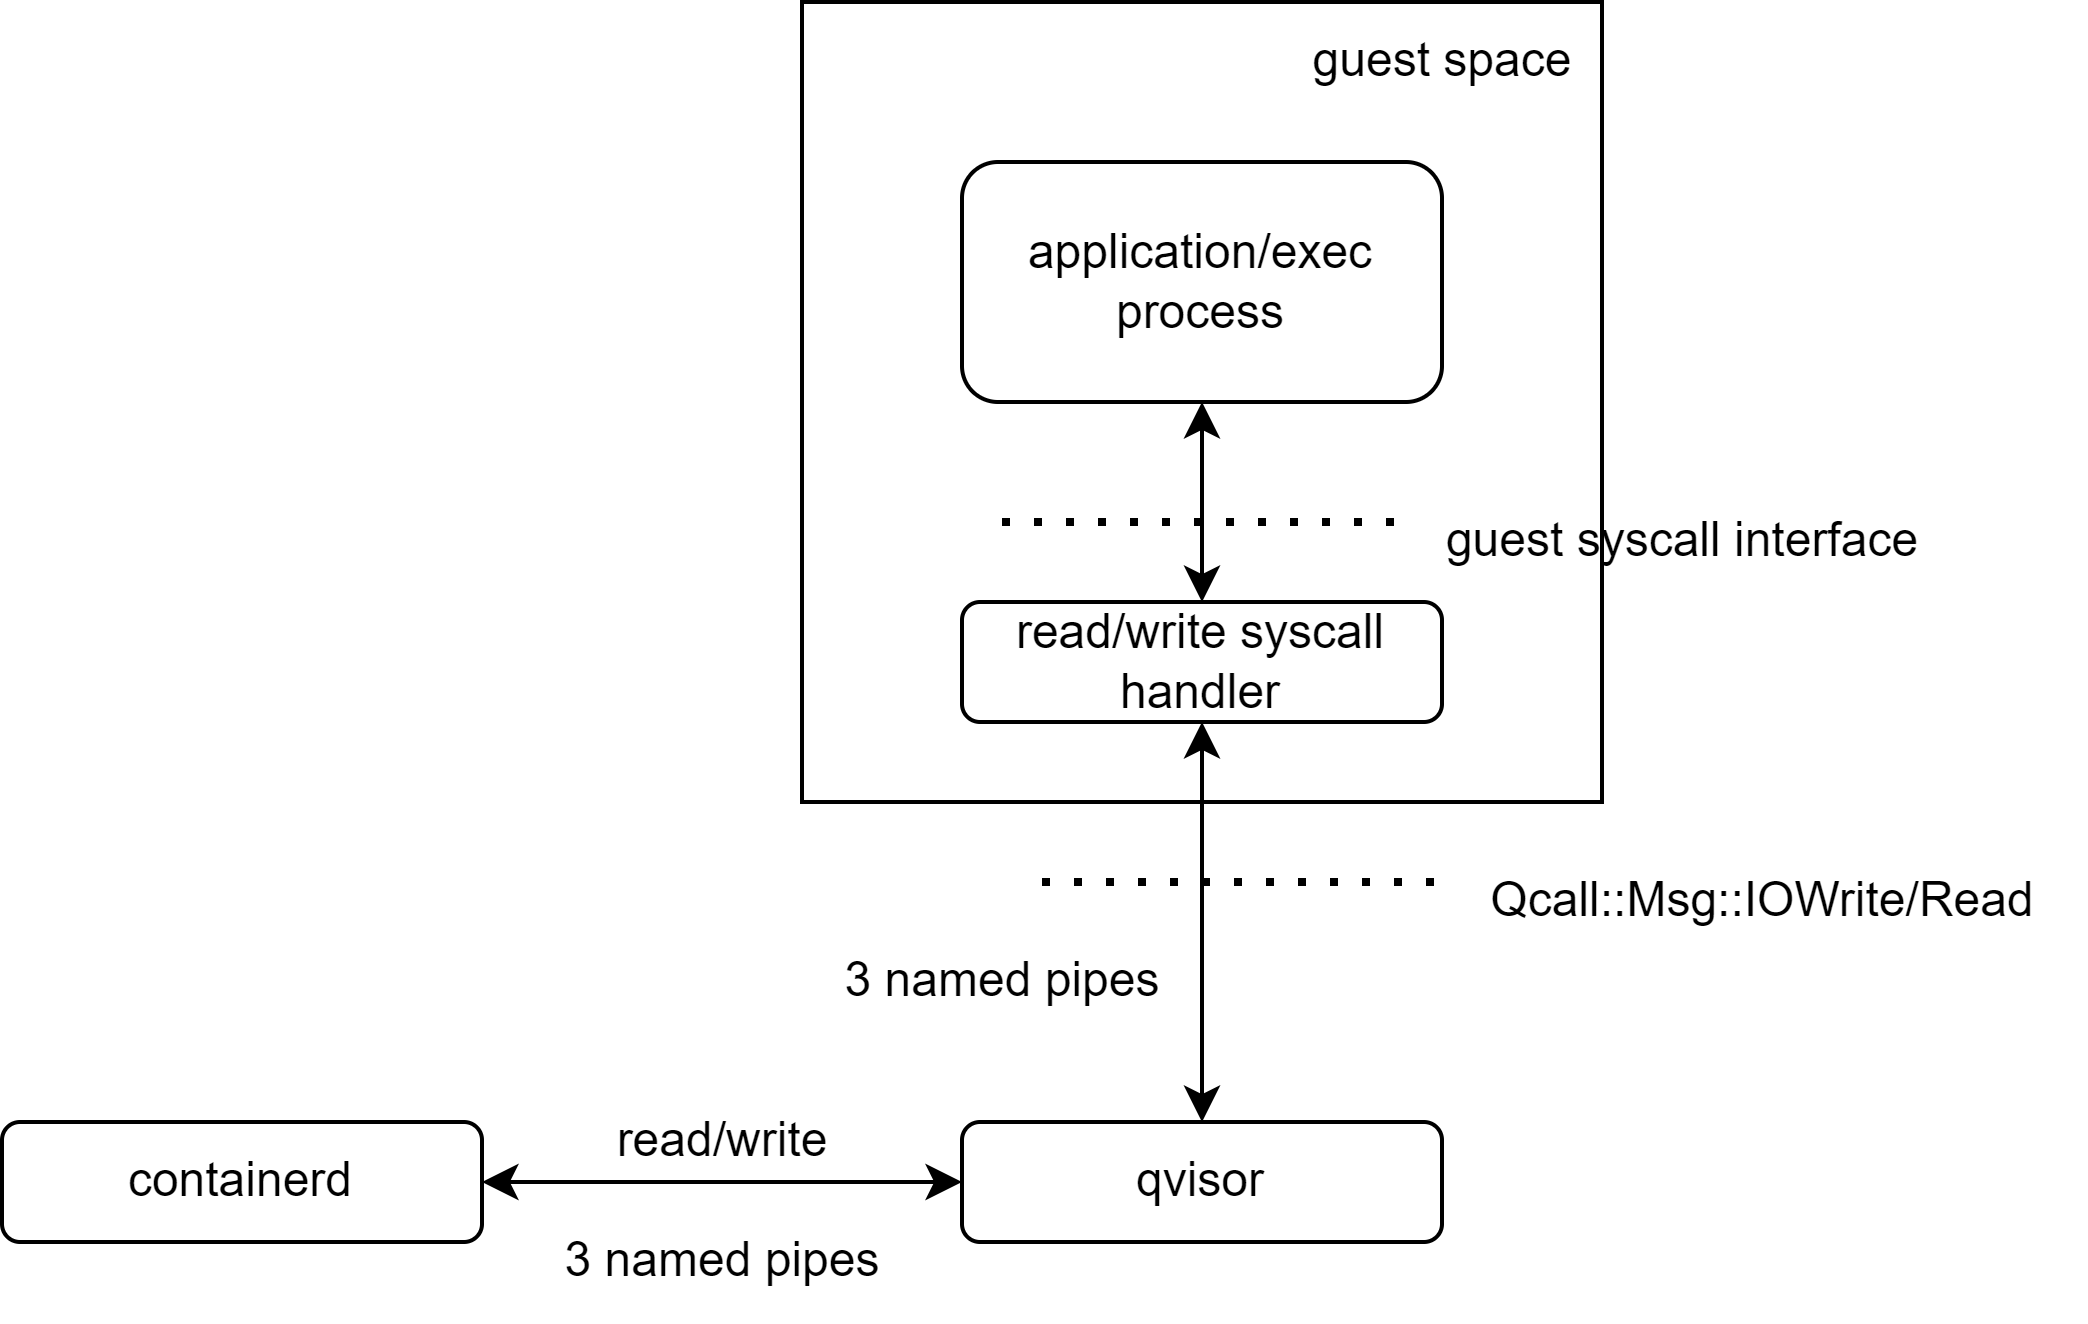
\includegraphics[width=0.9\linewidth]{images/normorl_io.png} 
      \caption{Normal IO} 
      \label{fig1:a} 
      \vspace{4ex}
    \end{subfigure}%% 
    \begin{subfigure}[b]{0.5\linewidth}
      \centering
      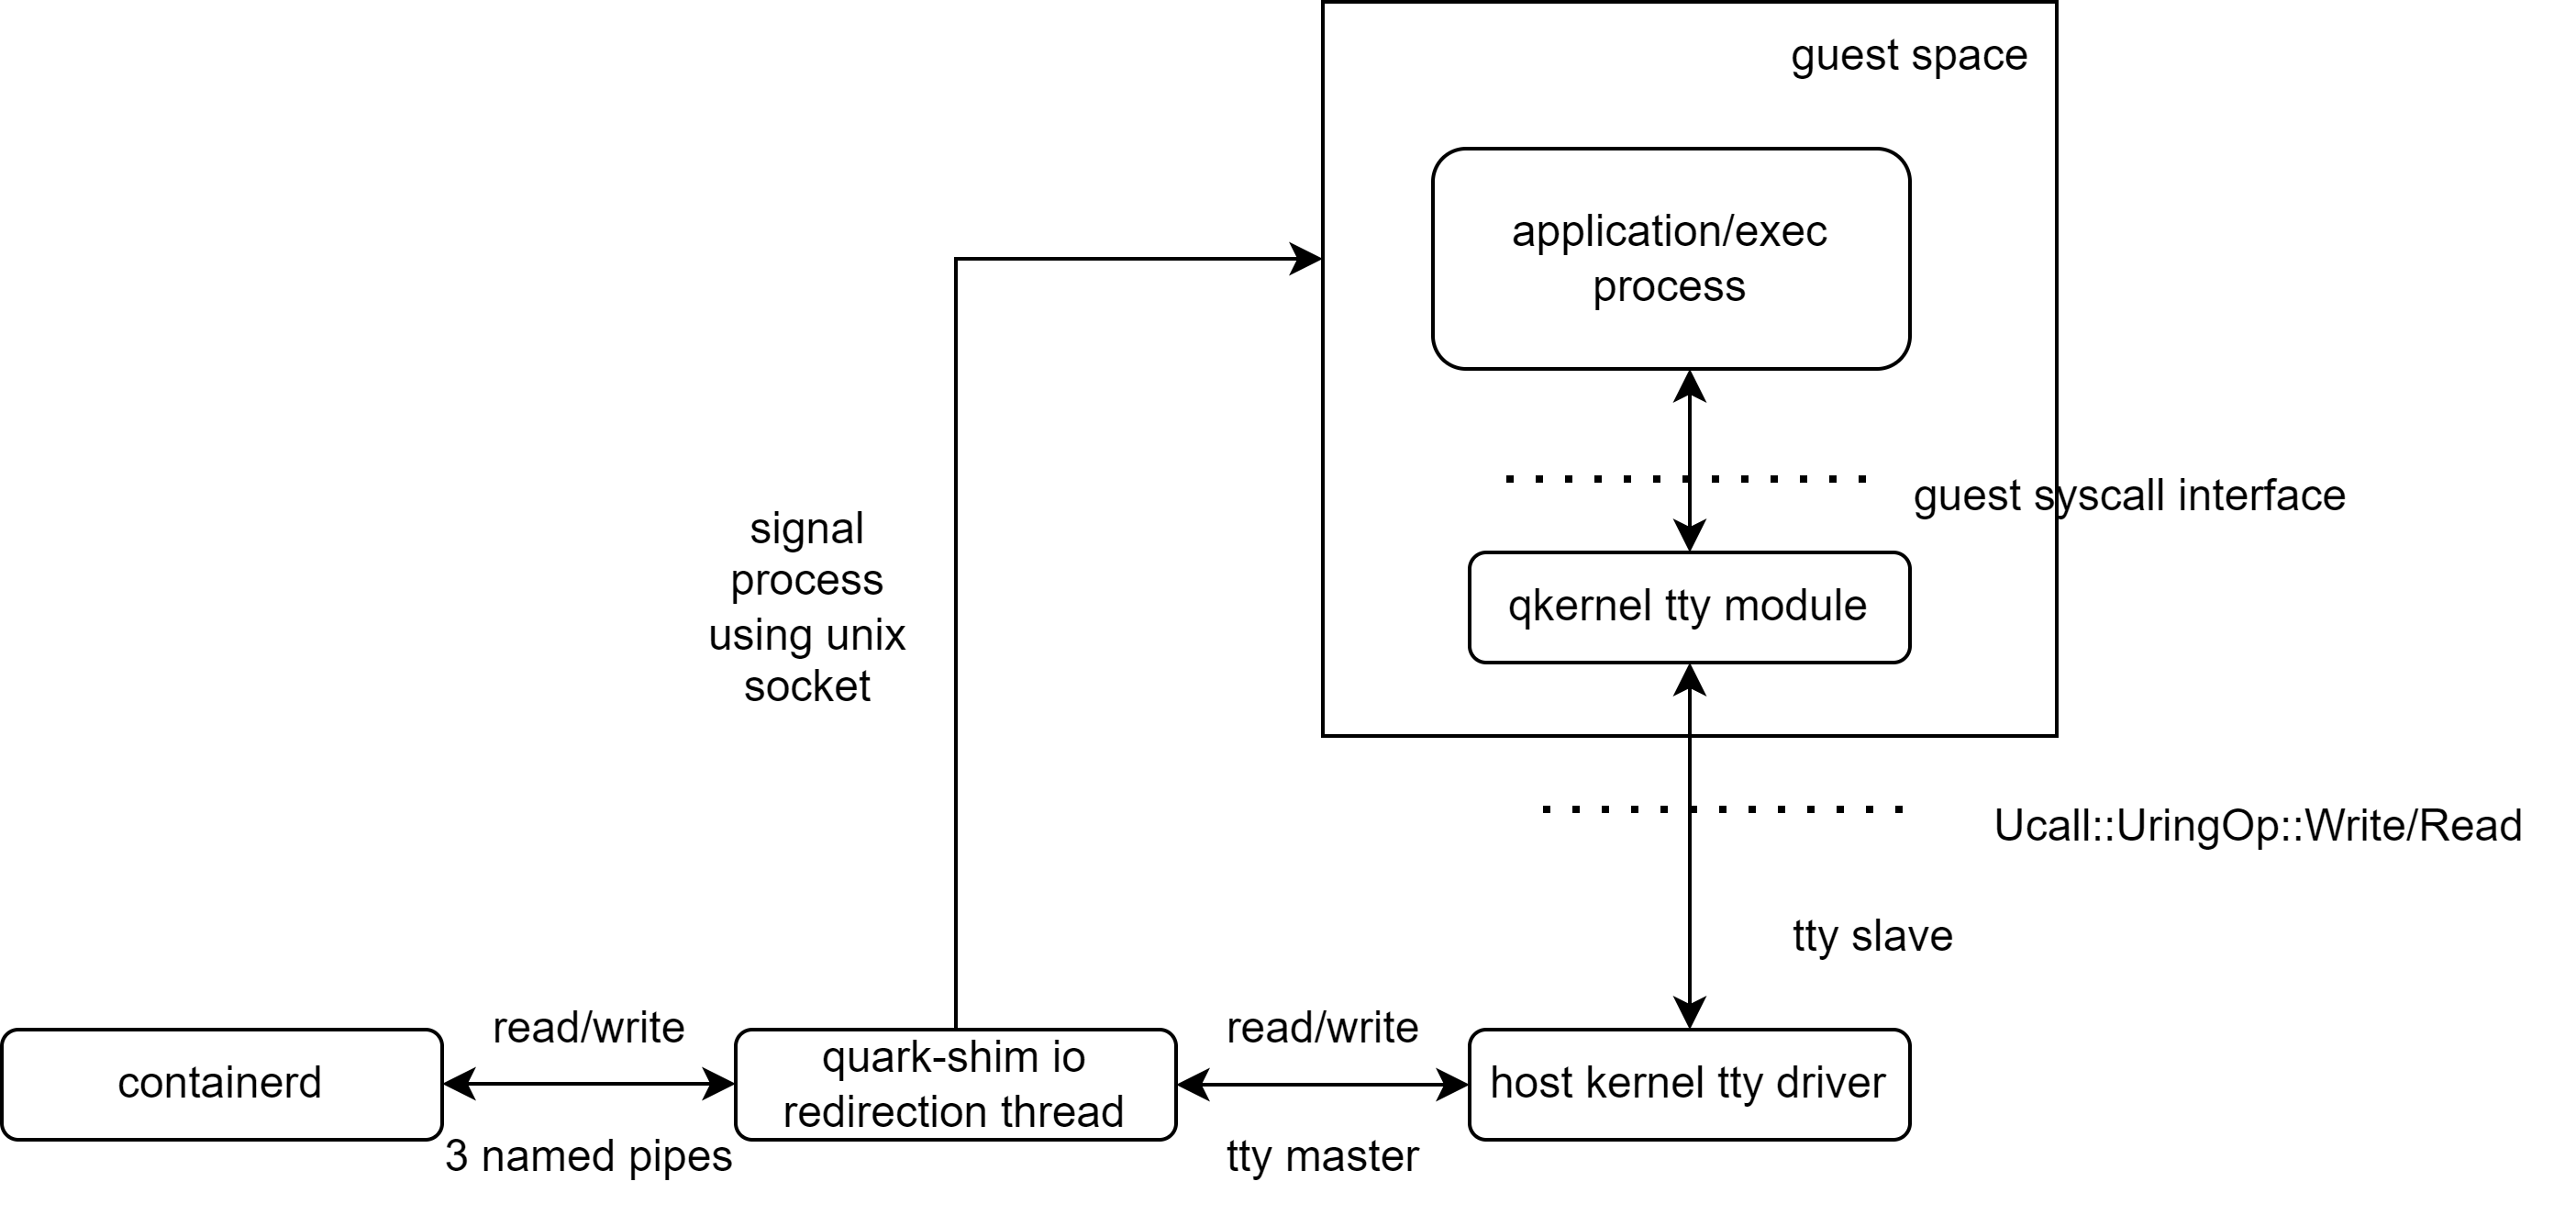
\includegraphics[width=0.9\linewidth]{images/termianl_workflow.png} 
      \caption{Terminal IO} 
      \label{fig1:b} 
      \vspace{4ex}
    \end{subfigure} 
    \caption{Guest User Space Process STDIO Handling Workflow}
    \label{fig1} 
\end{figure}


The Quark handles the process's STDIO differently based on the terminal keyword in the specification.  
When the terminal keyword is true, Quark-shim creates an asynchronous terminal IO redirection thread and a TTY pair (TTY master and TTY slave). The  TTY slave is then sent to the Quark-agent, where it is set as stdin, stdout, and stderr of the 
process. The redirection thread (as illustrated in Figure~\ref{fig1:b}) filters the signals in the STDIN-named pipe and transfers the data between the tty master and the named pipes. The filtered signals include SIGINT, SIGQUIT, and SIGTSTP, 
which are forwarded to the Quark agent via the Unix socket. The Quark agent will signal the process accordingly. For instance, when the character \verb|^C| (ASCII code 3) appears in the STDIN-named pipe, the redirection thread sends SIGINT to the 
process, ultimately terminating it. Furthermore, the Qkernel manages the tty slave by implementing a tty module. This module reads and writes the TTY slave through the UCLL interface. The data written to TTY master and slave are processed by the host
kernel TTY drive. It is responsible for character echoing, automatic translate each line feed (\textbackslash n) into a carriage return followed by a line feed (\textbackslash r\textbackslash n) in the data from TTY slave, and data buffering for 
data from TTY master. In this case, when the user presses enter (\textbackslash r), the driver moves the data for the buffer to the TTY slave. Note that the terminal works only when the guest user process's stdin is interactive, i.e., the stdin must 
be a TTY slave.  Conversely, when the terminal keyword is false, Quark-shim directly sends the three named pipes to the Quark agent, which then creates the exec process and uses the three named pipes as standard input, out, and error. Unlike the former case, 
Qkernel uses the Qcall interface for STDIO data transmission (Figure ~\ref{fig1:a}). 

While the process is running, Containerd~\cite*{containerd} will keep the three named pipes open. For the application process, stdout and stderr stream output are saved as log information to a location specified by Kubernetes. For the exec process, 
command execution results are returned to the user via stdout or stderr.

\textbf{End-to-end encryption for terminal data streams is missing.} When the terminal keyword is true in a process specification, the STDIO of exec or application processes is of the terminal type. The way untrustworthy Quark- shim process terminal 
IO threatens the confidentiality and integrity of the application data. In computer security, man-in-the-middle attack\cite*{Man_in_the_middle_attack} is a common attack mode where an attacker can intercept and forward messages between two parties to eavesdrop or alter 
communications. In the case of Quark, the attacker can use Quark-shim as a man-in-the-middle to intercept confidential data while the terminal redirection thread forwards the data. In severe cases, the attacker can change the commands the application 
owner sends or tamper with the command results to achieve their ulterior motives.


\textbf{Lack of cryptographic protection for application log}. The standard output and standard error stream data generated by applications are managed uniformly as application logs by Kubernetes. However, this approach is inappropriate since our 
threat model does not trust the cloud provider. An individual with cluster access can use the" kubectl logs pod-name" to view the application logs. Furthermore, A malicious administrator can log into the host running the application and view the 
application logs stored in the host file system. As a countermeasure, Qkernel should encrypt the application stdout and stderr stream data. Specific mitigation measures can be found in Section~\ref{sec:design_STDIO_PROTECTION}


 When the application owner issues commands to the application, the returned execution results are often confidential and sensitive. However, these results are returned by untrusted entities 
such as qvisor and containerd (as shown in Figure 3). For instance, if the application owner issues the command "cat /var/log/confidential.log" to the application, the Quark-agent would create a process to execute the "cat" binary and write the 
result to the process's stdout. Notably, the process’s STDIO in this case is set to named pipes. Subsequently, the qkernel's write syscall handler requests the Qvisor through Qcall to write the result to the named pipe, from where the Containerd 
gets the result and sends it back to the user. This setup gibe both Qvisor and Containerd the ability to temper with the command's results. As such, it is crucial to cryptographically protect the stdout and stderr of processes that execute commands 
from application owner. Further details on the mitigation measures can be found in Sections XX.

\textbf{Lack of cryptographic protection of exec request results.} When the application owner issues commands to the application, the returned execution results contain sensitive data. However, these results are returned by untrusted entities, i.e., 
Qvisor and Containerd (as shown in Figure~\ref{fig1:a}).   For instance, if the application owner issues the command" cat /var/log/confidential.log" to the application, the Quark agent would create a process to execute the" cat" binary and write the 
result to the process's stdout. Notably, the process's STDIO is set to named pipes in this case. Subsequently, the Qkernel's write syscall handler requests the Qvisor through Qcall to write the result to the named pipe, from where the containerd 
gets the result and sends it back to the user. This setup allows both Qvisor and Containerd to temper with the command's results. As such, it is crucial to cryptographically protect the stdout and stderr of processes that execute commands from the 
application owner. Further details on the mitigation measures can be found in Sections XXsssssssss.


\subsection{Issuing command and Terminal Allocation}
\textbf{Anyone can issue commands to an application.} Currently, the Quark agent (see section~\ref{sec:security_analyse_STDIO} for an explanation) in the qkernel lacks authentication and access control on the EXEC requests sent from the Quark shim. 
Therefore, an adversary can issue commands to the application to collect the application's sensitive data. An example of such access can be illustrated by executing kubectl exec pod-name printenv to obtain the application's environment variable 
type secret. In response to this vulnerability, we have classified the exec commands into two categories: "privileged" commands issued by the application owner and "unprivileged" commands issued by other users. Before executing these commands, the
Quark agent operates according to the least privilege principle to authenticate and access control on the exec requests. Therefore, unauthorized requests will be denied. For further details, please refer to section~\ref{sec:design_EXEC_Requests}.


\textbf{The privileged commands may contain confidential data but are unprotected during transmission.} Currently, the commands are sent to Quark shim by Containerd~\cite*{containerd} as part of the exec request's metadata via the shim- v2 API~\cite*{shim_v2}. 
Quark-shim processes the exec request similar to that used to create an application process. When Quark-shim receives an exec request, it generates a process specification based on the metadata. This specification includes the command to be executed 
and the STDIO type. Quark shim forwards this specification to the Quark agent via a Unix socket. The Quark agent then creates a guest userspace process to execute the command (see Figure~\ref*{fig:quark_agent_work_flow}). However, As 
Quark-shim and Containerd are untrusted, the commands may be compromised or modified during transit. To this end, we should apply end-to-end cryptographic protection for privileged commands. The encryption occurs at the user end and decryption 
at the Qkernel side, preventing commands from unauthorized access during transmission. For additional information, see section~\ref{sec:design_EXEC_Requests}.


\textbf{Any user can allocate a terminal in Kubernetes using one of two methods:}

\begin{itemize}
  \item Creating a terminal process within a pod by using kubectl exec -it pod-name.
  \item Setting stdin: true and tty: true in the container specification during interactive application deployment and then attaching to the application process's stdio using kubectl attach-it pod-name~\cite*{Understanding_sdin}.
\end{itemize}


For Quark-shim and Quark-agent, this means that the keyword terminal is set to true in the process specification. In this case, the Quark agent treats the process stdio as terminal, as explained in section XXXXX. However, the Quark agent does not 
validate the keyword terminal when creating processes, and this may lead to unauthorized access:

any user can attach to an interactive application, then issue commands. Unlike EXEC requests, the attach requests are processed by Containerd~\cite*{containerd}. In this case, Containerd creates an IO redirection thread that transfers data between 
the STDIO of the user-side process and the three named pipes in Containerd representing the STDIO of the application. As a countermeasure, the easiest way is to encrypt the stdout and stderr of the application. With this approach, even if an 
attacker attaches to the application, the terminal cannot be used appropriately because the attacker does not possess the key to decrypt the application process's stdout and stderr stream. For more details, please refer to section~\ref{sec:design_STDIO_PROTECTION}.


On the other hand, any user with access to the cluster can use the kubectl exec -it to allocate a terminal. This allows an attacker to issue arbitrary commands to an application without restriction. In this case, Quark-agent creates a process based 
on the process specification of the EXEC request and sets the process STDIO to the terminal type. As a countermeasure, the Quark agent should follow the least privilege principle to verify that this user has permission to set the STDIO to the 
terminal type before creating the process. For further information, please see section~\ref{sec:design_EXEC_Requests}.


% the qkernel should measure the terminal keyword in the application 
% process specification before creating the process. The measurement should then be sent as part of the application's startup hash to the relying party. In this way, the relying party ensures that the stdio of the application is of the correct type.  

\subsection{Paravirtualized File System Sharing}

The application accesses the rootfs on the host system through the Paravirtualized File System Sharing mechanism.   In creating the application, Quark-shim first generates a mount namespace for the Quark sandbox. It then utilizes the information in 
the application bundle to mount the rootfs of the application into the Quark sandbox path, thus making it available to the Qkernel. During runtime, the application accesses the rootfs on the host system through the Qkernel para-virtualized file 
system sharing mechanism. For instance, when the application utilizes the guest-read system call to access a file in the rootfs, the guest-read system call handler will request the host to read the target file via Hypercall or Ucall interface. 
In response, the host kernel processes the request and shares the outcome with the application via the interface above.


\begin{figure}[ht] 
  \begin{subfigure}[b]{0.5\linewidth}
    \centering
    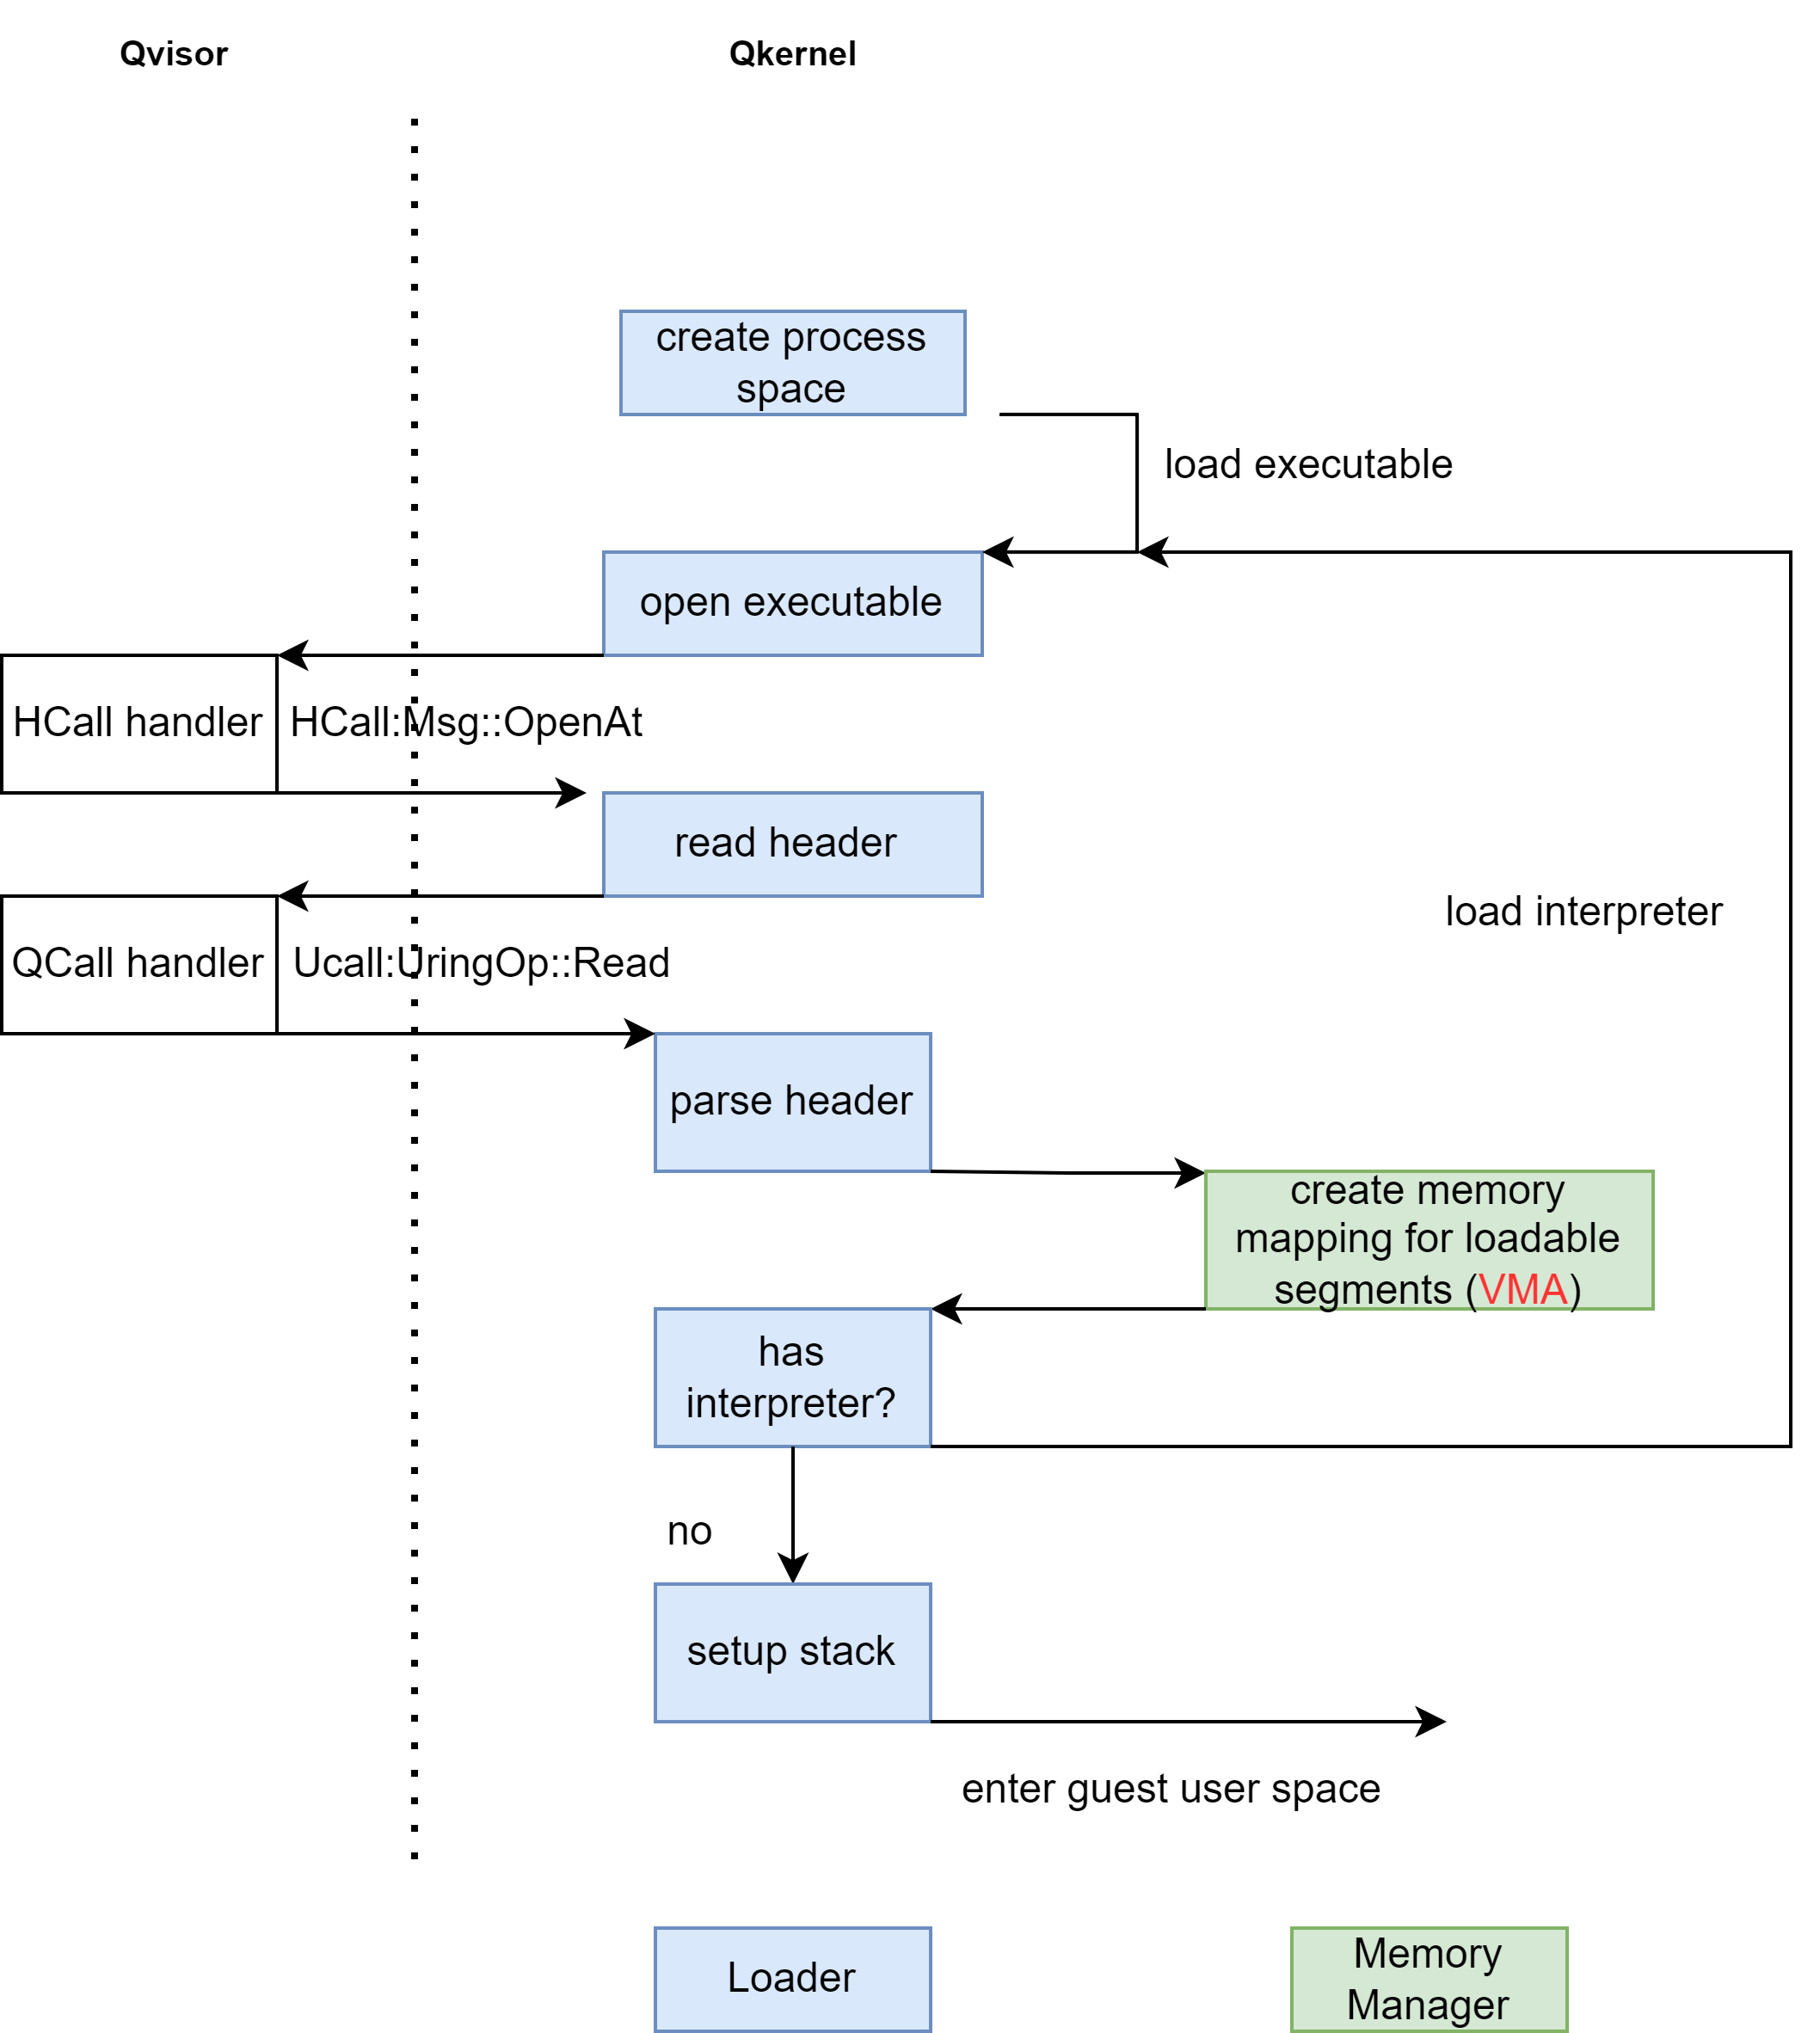
\includegraphics[width=0.9\linewidth]{images/loader_flow.png} 
    \caption{Loader setup Memory Mappings during Application Startup} 
    \label{fig2:a} 
    \vspace{4ex}
  \end{subfigure}%% 
  \begin{subfigure}[b]{0.5\linewidth}
    \centering
    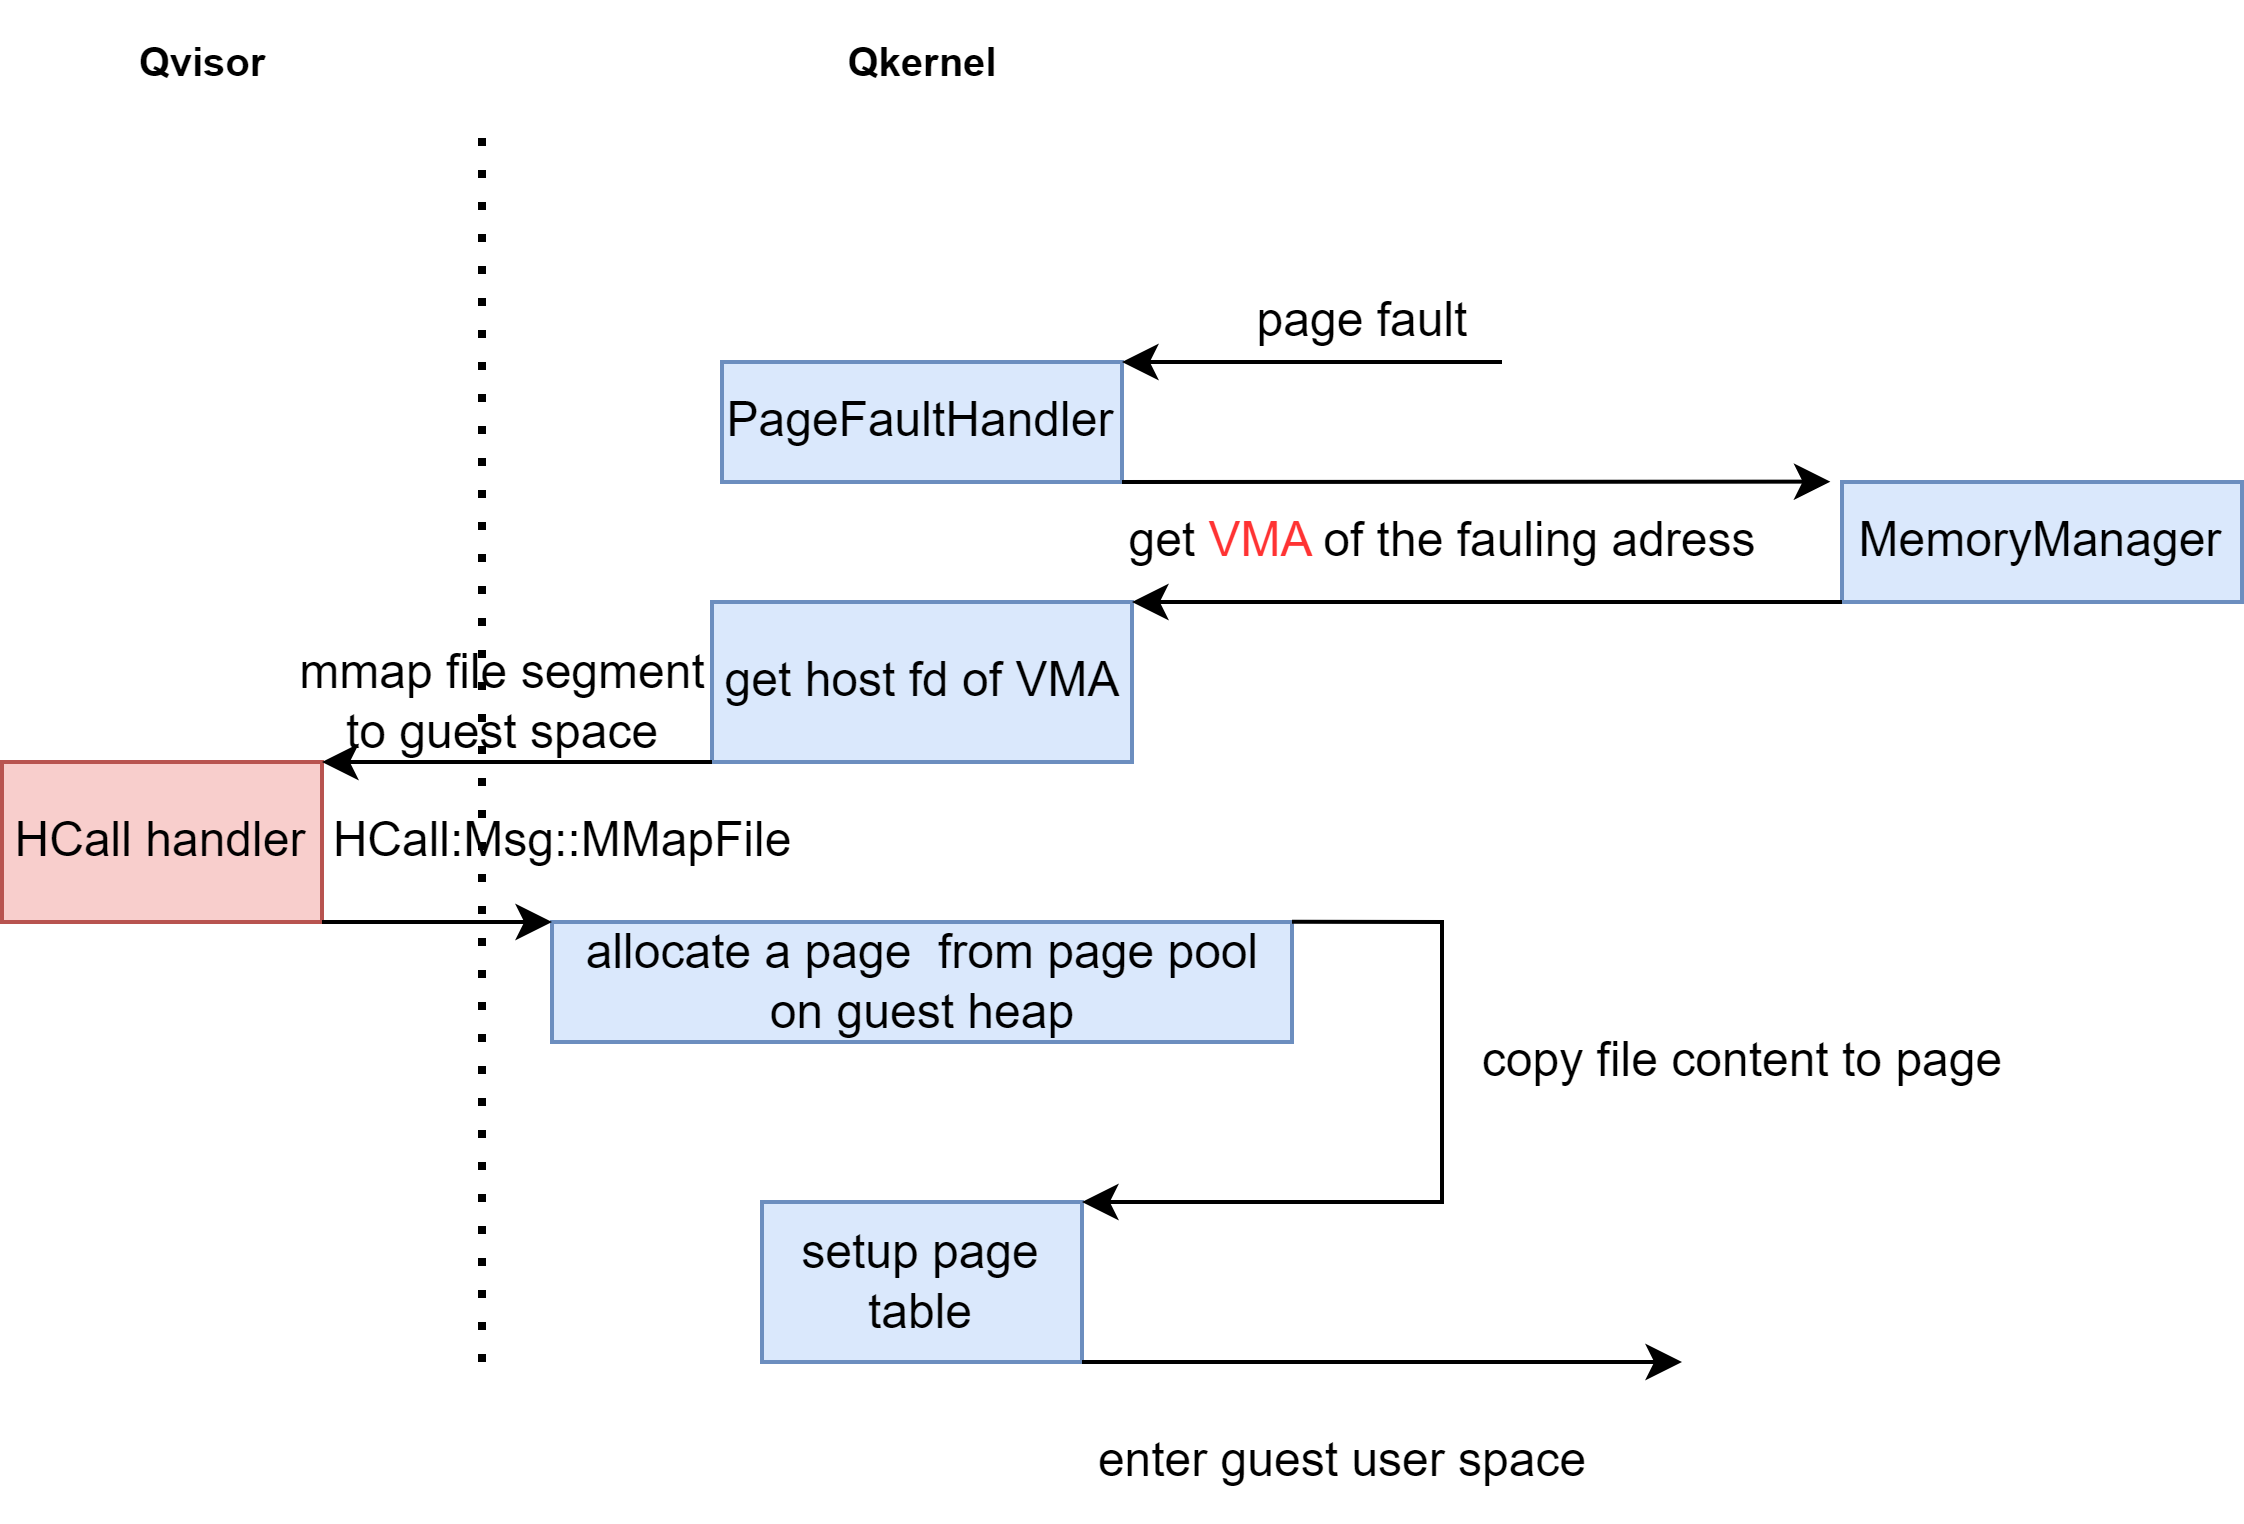
\includegraphics[width=0.9\linewidth]{images/page_fault_handling.png} 
    \caption{Page Fault Handling} 
    \label{fig2:b} 
    \vspace{4ex}
  \end{subfigure} 
  \caption{Application Binary Loading Process}
  \label{fig2} 
\end{figure}

\subsubsection{Loading compromised application binary during startup}
\label{sec:app_binary_loading}
The application binary is stored in the host’s space. During the setup of the application process, the Qkernel loader opens the application binary using Hcall::Openat, reads its ELF header into the Qkernel using the Ucall::read, and then requests 
the Qkernel virtual memory manager to create a process image for the application. The memory manager creates a private virtual memory area (VMA) for each loadable segment defined in the ELF file  (Figure~\ref{fig2:a}). When the application process 
runs, accessing an address within the VMA will trigger a page fault. This is handled by the qkernel page fault handler. 

The workflow for the page fault handling can be found in Figure~\ref{fig2:b}. Since the VMA of a loadable segment is private, the page fault handler uses hcall::mmap to request Qvisor to map the relevant loadable segment into the guest physical space, 
then allocate a page from the page pool on the Qkernel heap, and copies the contents of the segment from the guest physical address to this page. Finally, a page table entry (guest virtual address -> address of the page) is created. After this, 
the page fault handler hand over the control to the guest user process. 

The fact that the application binary is loaded from the host makes it possible for an attacker to induce Qkernel to execute compromised codes. For instance, the loader might request Qvisor to open binary A using Hcall::openat, but instead, 
untrusted Qvisor provides the descriptor of file B. As a result, the loader creates the wrong memory mapping. Consequently, the page fault handler will load the code from file B instead of file A. Furthermore, since the page fault handler uses 
Hcall::mmap to map the executable into the guest physical space, an attacker could manipulate the Qvisor to map compromised code. In this case, the page fault handler simply copies this code to a page, creates a page table entry, and then returns 
to the application process without an integrity check. This leads to the execution of malicious code. 

To mitigate this vulnerability, after the memory manager creates a VMA for a loadable segment, the Qkernel should immediately read the address range. This facilitates the page fault handler to load the segment into the guest before the application 
runs. Also, the Qkernel should measure the read content simultaneously. The measurement result should be sent to a relying party for integrity checking. In this way, we ensure the correctness of the application binary loaded into the qkernel.



\begin{figure}[H]
  \centering
  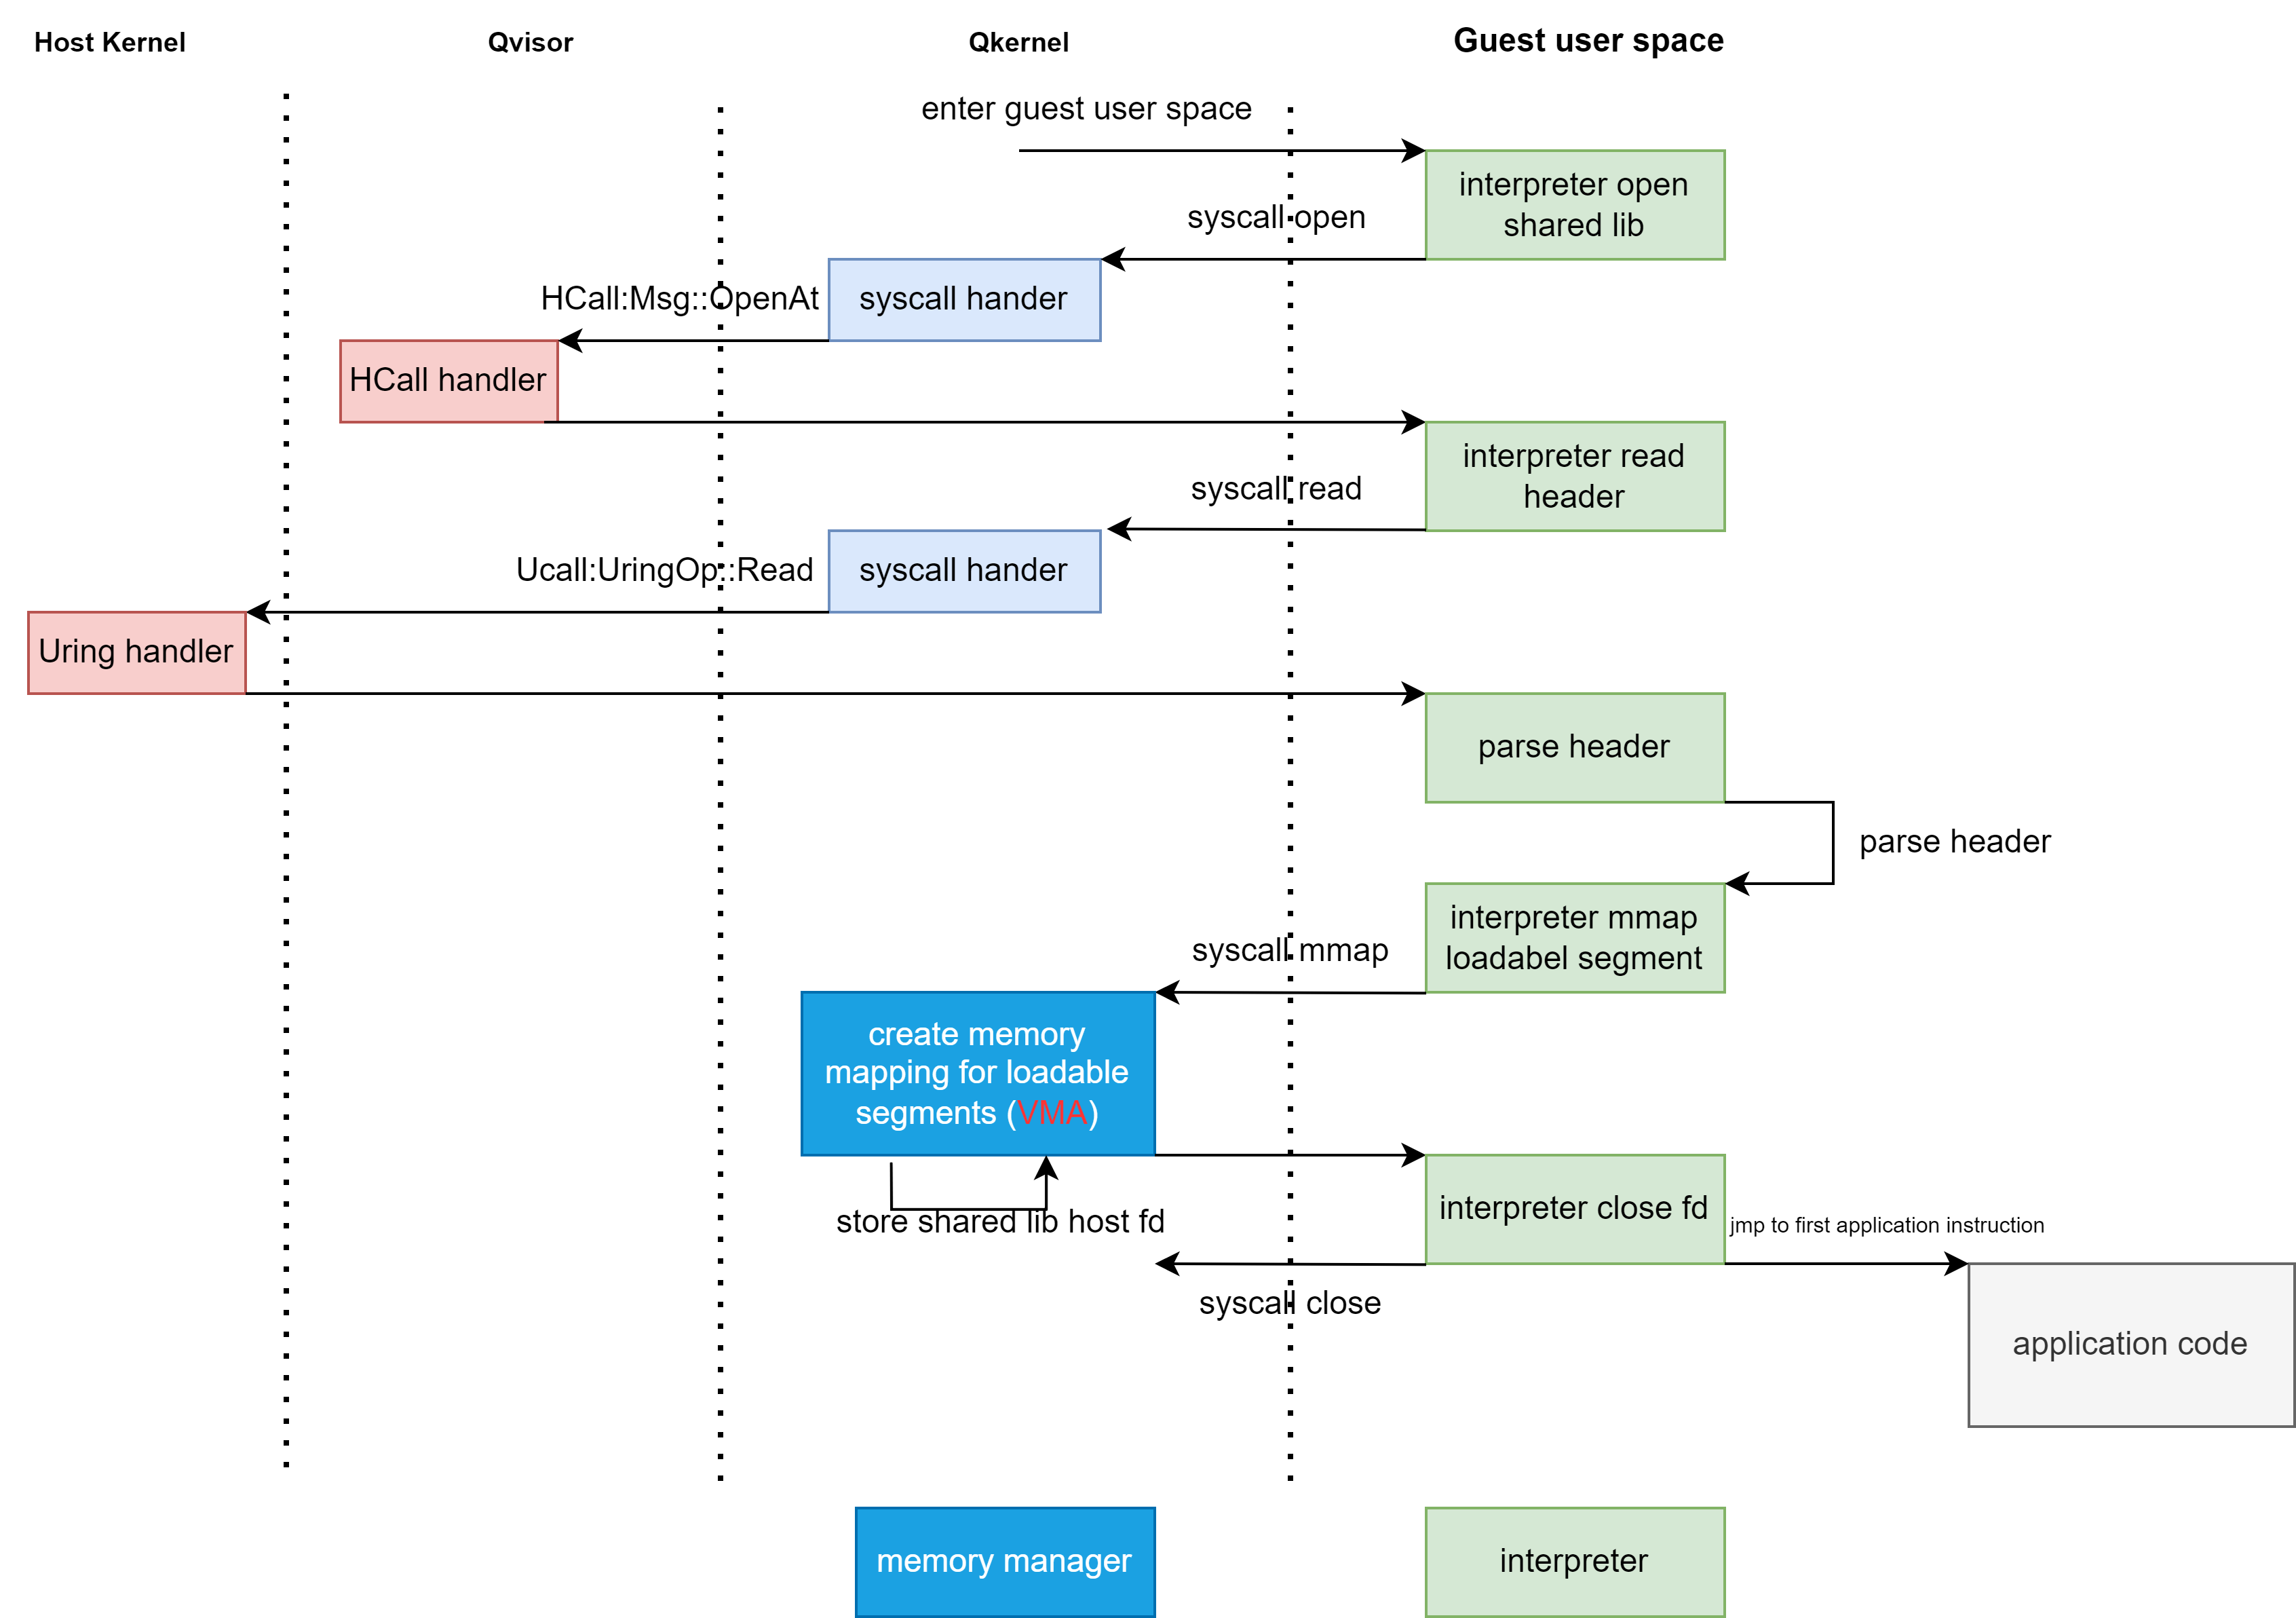
\includegraphics[width=1\textwidth]{images/load_shared_libarart.png}
  \caption[Interpreter setups shared library's memory mappings]{Interpreter setups shared library's memory mappings}
  \label{fig:load_shared_libarart}
\end{figure}


\subsubsection{Loading compromised binary at runtime}
Dynamic libraries are binary files stored on the host and loaded at application runtime by the interpreter. When the application is a dynamically linked executable, the interpreter’s code is executed upon launching the application process. 
As depicted in Figure~\ref{fig:load_shared_libarart}, the interpreter uses the open, read, and mmap system calls to create private memory mappings (VMAs) for the loadable segments in a shared library. Accessing an address within the VMAs triggers 
page faults. The page fault handler handles the fault like how it handles page faults when accessing the VMA of the application binary. 

Since the process of how the Qkernel creates memory mapping and later loads code to the guest for shared library and application binary are very similar, the issues encountered in the previous section also apply here. To this end, the Qkernel should 
measure the shared library by reading the VMA before the mmap system call is returned. This prompts the page fault handler to load the library into the guest. However, since the library’ measuring happens after remote attestation, the Qkernel does 
not forward the measurements to the relying party. Instead, it verifies these measurements against the reference hash in the policy file obtained from the relying party.

Executing a command at runtime will cause the qkernel to load the binary corresponding to that command. For example, for the exec command, the quark-agent will load the binary corresponding to the command and create a process. The binary loading 
mechanism has already been discussed in section~\ref{sec:app_binary_loading}.   Therefore, a malicious user can inject malicious code into the Qkernel. The mitigation is similar to the previous section, where Qkernel measures the binaries loaded into Qkernl and checks 
the correctness of the loaded binaries using the reference hashes in the policy file obtained from the relying party.


\subsubsection{Lack of management of application restarts}

In the event of an unexpected application crash, Kubernetes may recreate a pod to execute the crashed application or restart the program within the original pod if the persists. In the latter case, Qkernel reloads the application binaries 
and process specifications. from the host and provide the relaunched application with the secret obtained from relying party during the first startup. An attacker may use this opportunity to inject malicious code and process specifications into Qkernel, 
which causes an incorrect process setup or executing of compromised code. To mitigate this threat, Qkernel should measure the application recreation process and compare the measurement result with the initial application startup measurement stored 
on guest memory. If the 2 hashes don’t match,  Qkernel should panic.

In an unexpected application crash, Kubernetes may recreate a pod to execute the crashed application or restart the program within the original pod if it still exists\cite*{k8s}. In the latter case, Qkernel reloads the application binaries from the host 
and provide the application with the secret obtained from relying party during the first startup. An attacker may use this opportunity to inject malicious code into Qkernel, which causes the execution of compromised code. To mitigate this threat, 
Qkernel should measure the application recreation process and compare the result with the initial application startup measurement stored on guest memory. If the two hashes do not match, Qkernel should panic.

\subsection{No restriction to the available System Calls for Applications}

The seccomp section in the OCI runtime specification\cite*{oci-spec} defines a way to restrict the available system calls for applications. Unfortunately, Qkernel does not support seccomp\cite*{seccomp}. If a guest process is compromised, a vulnerable 
system call can be abused to attack the qkernel and other processes. In computer security, component hijacking\cite*{DBLP:journals/corr/WuGLD16} is an attack pattern in which an attacker can attack the kernel and other processes by hijacking a 
process and forcing it to execute a vulnerable system call. For example, an attacker can start a malicious EXEC process,  which uses a vulnerable system call to steal application secrets stored in Qkernel. 

To this end, we implement a guest system call interceptor. The application owner can specify the available system calls for an application. For more details, please refer to section~\ref*{sec:design_Interceptor}.

\subsection{No control over guest kernel arguments}
\begin{figure}[H]
  \centering
  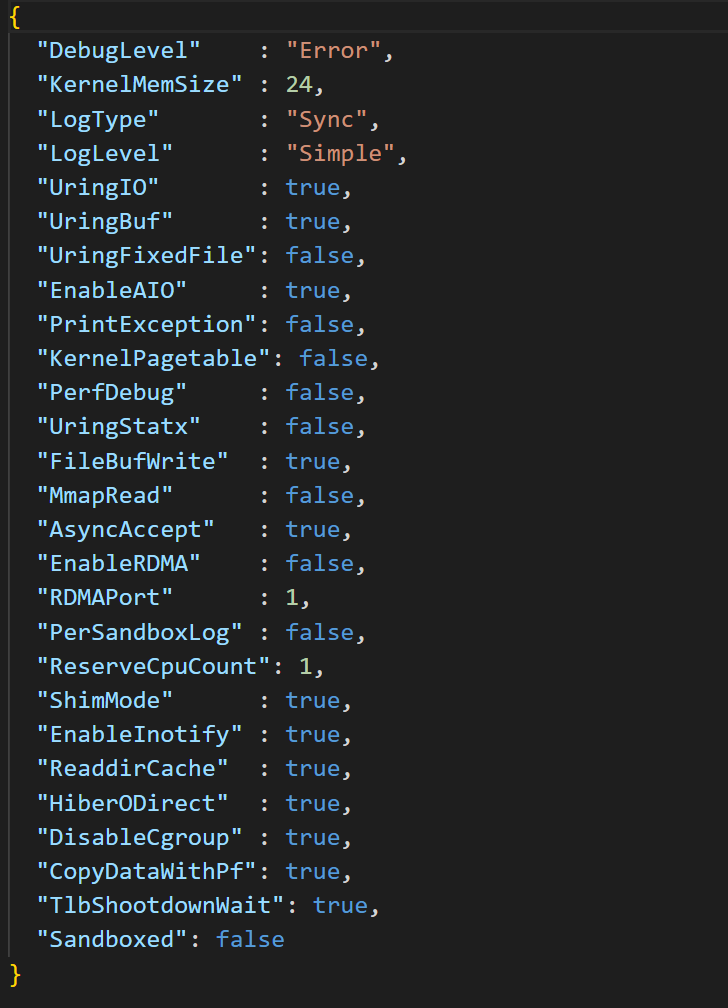
\includegraphics[width=0.5\textwidth,height=0.4\textheight]{images/quark_config.PNG}
  \caption[Configuration file for Qkernel, Qvisor, and Quark shim]{Configuration file for Qkernel, Qvisor, and Quark shim. The file is installed as a global configuration file for quark in the /etc/quark/ directory. When quark-shim or qvisor starts, it reads this file and completes the relevant configuration}
  \label{fig:quark_config}
\end{figure}

Qkernel is a binary loaded into the guest memory during Qvisor setting up the guest. To properly configure the Qkernel, Qvisor also passes several command-line arguments to the Qkernel, including the number of VCPUs, the socket file descriptor that 
the Quark-agent listens to, and a configuration file shown in Figure~\ref{fig:quark_config}. This configuration file specifies the runtime behavior of the Qkernel, such as whether to enable the Ucall interface, whether to enable RDMA, etc. A wrong configuration file 
can lead to the disclosure of the secrets stored in Qkernel. For example, turning on RDMA would allow an untrusted party direct access to the Qkernel’s memory. For this reason, the Qkernel should measure the configuration file and send it to the relying party for integrity checking.

\subsection{Qkernel Log Misconfiguration}
\label{sec:Qkernel_Log_Misconfiguration}

Qkernel logs are stored by qvisor in the host /var/log/quark directory via Hcall::HYPERCALL\_PRINT. Currently, the Qkernel logging system supports five logging levels: OFF, Error, Info, Debug, and Trace. Here OFF is the minor level, i.e., 
the least detailed, and Trace is the highest level, i.e., the most detailed log. The user can configure the highest level of logging for qkernel through DebugLevel keyword in the configuration file (Figure~\ref{fig:quark_config}). For example, when 
the DebugLevel is Info, qkernel prints logs in level Error, and Info. A malicious administrator may set the DebugLevel keyword to Trace and then analyze the Qkernel logs to obtain sensitive information. 

This problem can be solved by measuring the guest kernel arg. However, both Qvisor and Qkernel are configured using this file. Specifically, Qvisor reads this configuration file after startup and passes a copy into the Qkernel as a command line 
argument when launching the guest. Suppose the k8s administrator sets the DebugLevel keyword to trace to view the Qvisor’s logs. In this case, the Qkernel will have to print very detailed log messages, which may contain the application’s secrets. 
To break the coupling between the Qvisor and Qkernel logging system configuration, we should offload the Qkernel logging system configuration from this configuration file and allow the application owner to specify the Qkerenl maximum logging level 
in a policy. This policy is obtained at application startup via remote attestation. Until then, the logging level of the Qkernel is set to the default level OFF, i.e., no logs will be printed.




\section{Summary}
In this chapter, the threat model is first defined in section~\ref{sec:Threat_model}. Based on this model, the security issues in Quark are examined from various perspectives. These vulnerabilities found include:
\begin{itemize}
  \item Application secrets are managed and deployed by untrusted Kubernetes and Quark-shim
  \item Absence of end-to-end encryption for terminal data streams
  \item  Lack of cryptographic protection for application log
  \item Anyone can issue commands to an application
  \item Any user can allocate a terminal
  \item The commands issued by application owner may contain confidential data but are unprotected during transmission.
  \item Loading compromised application binary during startup
  \item Loading compromised binary/shared library at runtime
  \item Lack of management over application restart
  \item No restriction to the available system calls for applications
  \item No control over guest kernel arguments
  \item Guest kernel Log misconfiguration

\end{itemize}

% For this reason, we should offload the configuration of the logging system from the qkernel configuration file and allow the application owner to specify the maximum logging level for the specified client kernel logging system in the protection 
% policy.
\cleardoublepage

%%% Local Variables:
%%% TeX-master: "diplom"
%%% End:
